\documentclass[12pt,a4paper]{article}
\setlength{\textwidth}{160mm}
\setlength{\textheight}{247mm}
\setlength{\evensidemargin}{0pt}
\setlength{\oddsidemargin}{0pt}
\setlength{\topmargin}{0pt}
\setlength{\headheight}{0pt}
\setlength{\headsep}{0pt}
\usepackage{amssymb}
\usepackage{amsmath}
\usepackage[polish]{babel}
\usepackage[T1]{fontenc}
\usepackage[utf8]{inputenc}
\usepackage{graphicx}
\usepackage{algorithm,algorithmic}
\title{Algorytmy Graficzne}
\author{Patryk Wojciekian}
%\date{}
\begin{document}
\maketitle
\begin{abstract}
Algorytm — skończony ciąg jasno zdefiniowanych czynności, koniecznych
do wykonania pewnego rodzaju zadań. Sposób postępowania
prowadzący do rozwiązania problemu
\end{abstract}
\section{Algorytm de Casteljau}
\textit{Algorytm de Casteljau} - algorytm opracowany przez Paula de Casteljau,
pozwalający na wyznaczenie punktów na wielomianowej krzywej Beziera.\\
Dana jest dowolna łamana zdefiniowana przez $n + 1$ wierzchołków $p_0, p_1,
\dots , p_n$ oraz liczba $t \in [0, 1]$ Każdy odcinek łamanej jest dzielony w stosunku
$t : (1 - t)$, czego wynikiem jest n wierzchołków, które wyznaczają nową
łamaną. Proces powtarzany jest do chwili, aż zostanie jeden punkt $p(t)$, co
wymaga wykonania $n$ kroków. Ostatecznie otrzymuje się $n + 1$ ciągów punktów. 
(indeks górny oznacza krok algorytmu):
\begin{figure}[h!]
\centering
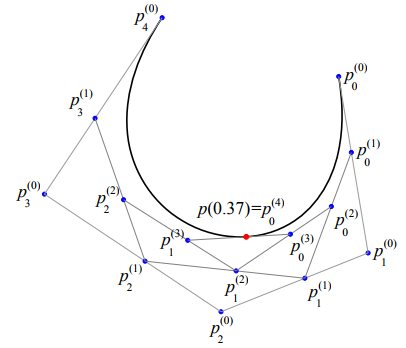
\includegraphics{obraz.png}
\caption{ Algorytm de Casteljau -- cztery kolejne łamane, na czerwono wynikowy
punkt $p(t) (t = 0,37)$. Kolorem czarnym narysowano krzywą Beziera,
na której leży $p(t)$}
\label{obraz1}
\end{figure}
\begin{gather*}
p_0^{(0)},p_1^{(0)},p_2^{(0)},\dots,p_{n-1}^{(0)},p_n^{(0)} \\
p_0^{(1)},p_1^{(1)},p_2^{(1)},\dots,p_{n-1}^{(1)} \\
\vdots \\
p_0^{(n-1)},p_1^{(n-1)} \\
p_0^{(n)} \\
\end{gather*}

Punkt $p(t)^{(n)}$ leży na krzywej Beziera, której \textit{łamaną kontrolną} tworzą wyjściowe punkty (rysunek \ref{obraz1})
\section{Lista kolorów}
Rozdział zawiera spis często używanych kolorów, zarówno w języku codziennym,
jak i w specyficznych grupach zawodowych. W tabeli \ref{kolory1} pogrupowano
nazwy barw alfabetycznie, z dołączoną próbką, a także opisem RGB i w systemie
szesnastkowym (Hex).

\begin{table}
\centering
\begin{tabular}{lccccl}
\textbf{Nazwa}&\textbf{HEX}&\textbf{R}&\textbf{G}&\textbf{B}&\textbf{Opis} \\ \hline
akwamaryna & \#7FFFD4 & 127 & 255 & 212 & „morska woda”\\
alabastrowy & \#FAFFFA & 240 & 255 & 240 & kolor minerału\\
amarantowy & \#E61C66 & 230 & 28 & 102 & szkarłatny\\
ametystowy & \#9966CC & 153 & 102 & 204 & purpurowofioletowy\\
antracytowy & \#364135 & 54 & 65 & 53 & szaro-czarny \\ \hline 
\end{tabular}
\caption{Lista kolorów alfabetycznie}
\label{kolory1}
\end{table}
\section{Algorytm Bresenhama}
\textit{Algorytm Bresenhama} służy do rasteryzacji krzywych płaskich, czyli do jak
najlepszego ich obrazowania na siatce pikseli. Jack Bresenham w 1965 roku
w artykule \cite{lit1} opracował metodę rasteryzacji odcinków, którą następnie
przystosowano do rysowania obiektów innego rodzaju (okręgów czy elips).
\subsection{Algorytm Bresenhama na okręgu}
\subsubsection{Założenia}
\begin{enumerate}
\item Promień okręgu ma długość $r$,
\item Rozważamy okrąg w I ćwiartce układu współrzędnych,
\item Środkiem symetrii okręgu jest środek układu współrzędnych,
\item Rysowanie okręgu zaczynamy od punktu $(0,r)$,
\item W każdym kroku stawiami symetrycznie 8 punktów okręgu,
\begin{itemize}
\item osią wiodącą jest oś $OX$,
\end{itemize}
\end{enumerate}
\subsection{Algorytm i jego działanie}
Przybliżany okrąg ma równianie:
$$
x^2+y^2-r^2=0
$$
O wyborze piksela decydować będzie wartość funkcji
$$
f(x,y)=4\left((x+1)^2+(y-\frac{1}{2})^2-R^2\right)
$$
w punkcie środkowym $M$ położonym pomiędzy alternatywnymi pikselami. 
Gdy osią wiodącą jest $OX$ oblicza się:
$$
F(M)=F\left(x_i+1,y_i-\frac{1}{2}\right).
$$
Przy wyborze następnego piksela $P_{i+1}=S$ czyli $x_{i+1}=x_i,y{i+1}=y_i-1$ wartość zmiennej decyzyjnej wynosi:
\begin{multline*}
d_{i+1}=F\left(x_{i+1}+\frac{1}{2},y_{i+1}-1\right) = \\
= b^2(x_{i+1}+1/2)^2+a^2(y_{i+1}-1)^2-a^2b^2=d_i-2a^2y_{y+1}+a^2.
\end{multline*}
Dany krok został zaimplementowany w linijce 5 algorytmu 1.
\begin{algorithm}
\caption{Algorytm Bresenhama}
\begin{algorithmic}[2]
\REQUIRE Środek okręgu jest w $(0,0)$, primień $R\in\mathbb{N}$
\ENSURE Okrąg został wyświetlony
\STATE $i\leftarrow 0$, $j\leftarrow R$, $f\leftarrow 5 - 4R$
\STATE writePixel$(i,j)$
\WHILE{$i\leq j$}
\IF{f>0}
\STATE $f\leftarrow f+8i-8j+20$;
\STATE $j\leftarrow j-1$;
\ELSE
\STATE $f\leftarrow f+8i+12$;
\STATE $a\leftarrow a\cdot b$;
\ENDIF
\STATE $i\leftarrow i+1$
\STATE writePixel$(i,j)$
\ENDWHILE
\end{algorithmic}
\end{algorithm}

\begin{thebibliography}{9}
\bibitem{lit1}  J. E. Bresenham: Algorithm for computer control of a digital plotter.
,,IBM Systems Journal'', vol. 4, no. 1, pp. 25–30 (1965).
\bibitem{lit2}  Michał Jankowski: Elementy grafiki komputerowej. Warszawa: Wydawnictwa
Naukowo-Techniczne, 1990.
\end{thebibliography}

\end{document}


